\documentclass[14pt,a4paper]{extarticle}
%\documentclass[12pt,a4paper]{article}

\usepackage[utf8]{inputenc}
\usepackage[ukrainian]{babel}


\usepackage{amssymb}
\usepackage{physics}


\usepackage[active]{srcltx}
\usepackage[final]{pdfpages}

\usepackage[hidelinks]{hyperref}

\usepackage{verbatim}
%%%%%%%%%%%%%%%%%%%%%%%%%%%%%%%%%%%%%%%%%%%%%%%%%%%%%%%%%%%%%%%%%%
%\pagestyle{empty}                     %нумерацiя сторiнок i т.д.
\pagestyle{headings}                   %нумерацiя сторiнок вгорi зправа i т.д.
%\renewcommand{\baselinestretch}{1.5}   %мiжстрiчковий інтервал
%\parindent=7.5mm                      %абзацний відступ
 \righthyphenmin=2                     %перенос 2 останніх букв
 \pagenumbering{arabic}
 \tolerance=400
 \mathsurround=2pt
 \hfuzz=1.5pt
%%%%%%%%%%%%%%%%%%%%%%%%%%%%%%%%%%%%%%%%%%%%%%%%%%%%%%%%%%%%%%%%%%
 \hoffset=-0.5cm        %+2.5cm -- вiдступ вiд лiвого краю
 \voffset=-1.5cm        %+2.5cm -- вiдступ зверху
 \oddsidemargin=0.1cm   %ліве поле
 \topmargin=0.1cm       %верхнє поле
 \headheight=0.5cm      %висота верхнього колонтитулу
 \footskip=1cm          %висота нижнього колонтитулу
 \headsep=0.3cm         %відступ від колонт. до тексту
 \textwidth=17cm        %ширина сторінки
 \textheight=25.5cm     %висота сторінки
%%%%%%%%%%%%%%%%%%%%%%%%%%%%%%%%%%%%%%%%%%%%%%%%%%%%%%%%%%%%%%%%%%
 \newcounter{e}
 \setcounter{e}{0}
 \newcommand{\n}{\refstepcounter{e} (\arabic{e})}
 
 \newcounter{pic}
 \setcounter{pic}{0}
 \newcommand{\pic}[1]{\refstepcounter{pic} \vspace{-0.3cm}\textit{Рисунок \arabic{pic}\label{#1}.}}
 
 \newcounter{tabl}
 \setcounter{tabl}{0}
 \newcommand{\tabl}[1]{\refstepcounter{tabl} \vspace{-0.3cm}\textit{Таблиця \arabic{tabl}\label{#1}.}}
 
 \newcounter{dod}
 \setcounter{dod}{0}
 \newcommand{\dod}[1]{\refstepcounter{dod} \textit{Додаток \arabic{dod}\label{#1}.}}
 
 \newcounter{defn}
 \setcounter{defn}{0}
 \newcommand{\defn}[1]{\refstepcounter{defn} \textbf{Означення \arabic{defn}\label{#1}.}}
 
 \newcounter{theorem}
 \setcounter{theorem}{0}
 \newcommand{\theorem}[1]{\refstepcounter{theorem} \textbf{Теорема \arabic{theorem}\label{#1}.}}
 
 \newcommand{\proof}{\textit{Доведення. \space}}
% \setcounter{page}{1}
% \setcounter{section}{1}
%%%%%%%%%%%%%%%%%%%%%%%%%%%%%%%%%%%%%%%%%%%%%%%%%%%%%%%%%%%%%%%%%%
 \newcounter{stali}
 \setcounter{stali}{0}
 \newcommand{\s}{\refstepcounter{stali} \arabic{stali}}

 \newcommand{\st}{C_{\s}}
 \newcommand{\stl}[1]{C_{\s \label{#1}}}

 \newcommand{\cd}{{} $$ \vspace{-0.3cm} $$ {}}
 
 \newcommand{\nb}[2]{\righthyphenmin=#2 #1 \righthyphenmin=2}

%%%%%%%%%%%%%%%%%%%%%%%%%%%%%%%%%%%%%%%%%%%%%%%%%%%%%%%%%%%%%%%%%%
 
 \newcommand{\tabboxl}[2]{\parbox{#1}{\vspace{0.1cm} #2 \vspace{0.1cm} }}
 
 
 \newcommand{\tabboxr}[2]{\parbox{#1}{\vspace{-0.3cm}
 		\begin{flushright} #2 \end{flushright} \vspace{-0.3cm} }}
 
 \newcommand{\tabboxc}[2]{\parbox{#1}{\vspace{-0.3cm}
 		\begin{center} #2 \end{center} \vspace{-0.3cm} }}
 
 
%%%%%%%%%%%%%%%%%%%%%%%%%%%%%%%%%%%%%%%%%%%%%%%%%%%%%%%%%%%%%%%%%%
 \begin{document}
	
 %\bibliographystyle{insrt}

 \thispagestyle{empty}

 \begin{center}
	\large
	Міністерство освіти і науки, молоді та спорту України \\
	Львівський національний університет імені Івана Франка \\
	Факультет прикладної математики та інформатики \\
	Кафедра обчислювальної матаматики
 \end{center}

 \vspace{45pt}

 \vfill

 \begin{center}
	{\Huge{Звіт}}\\
	{\large на тему:}
 \end{center}

 \begin{center}\Large
	\textbf{\emph{"Розв'язування задачі Діріхле-Неймана для рівняння Лапласа"}}
 \end{center}

 \vfill
 \vskip100pt

 \begin{flushleft}
	\hskip8cm 
	Виконали:
	\\ \hskip8cm 
	студенти 4-го курсу групи ПМп-41
	\\ \hskip8cm
	напрямку підготовки (спеціальності)
	\\ \hskip8cm
	113 -- ``Прикладна математика''
	\\ \hskip8cm
	Бугрій Б.О.
	\\ \hskip8cm
	Середович В.B.
 \end{flushleft}

 \begin{flushleft}
	\hskip8cm 
	Перевірив:
	\\ \hskip8cm
	ст. в. Гарасим Я.С.
 \end{flushleft}

 \vfill

 \begin{center}
	\large
	Львів - 2020
 \end{center}

 \newpage
 \thispagestyle{empty}
 \tableofcontents

 \newpage
 \thispagestyle{empty}
 \addcontentsline{toc}{section}{Вступ}
 \section*{Вступ}
 \begin{center}\end{center}
 літературний огляд \\
 хто розглядав розв'язування цієї задачі \\
 які процеси описує \\
 мета - розв'язати якимось методом \\
 огляд наступних розділів

 \thispagestyle{empty}
 \section{Постановка задачі}
		
	Припускаємо, що деяке двовимірне тіло задається двозв'язною областю $D \subset \mathbb{R}$ з досить гладкою границею що складається з внутрішньої кривої $\Gamma_1$ та зовнішньої $\Gamma_2$. 
	
	Нехай $D_1 \subset \mathbb{R}$ – обмеженна область з гладкою границею $\Gamma_1 \subset C^2$ та $D_2 \subset \mathbb{R}$ – обмеженна область з гладкою границею $\Gamma_2 \subset C^2$. Тоді двозв'язна область $D = D_2 \; \backslash \; \overline{D}_1$ матиме вигляд:

	\begin{figure}[h]
		\centering
		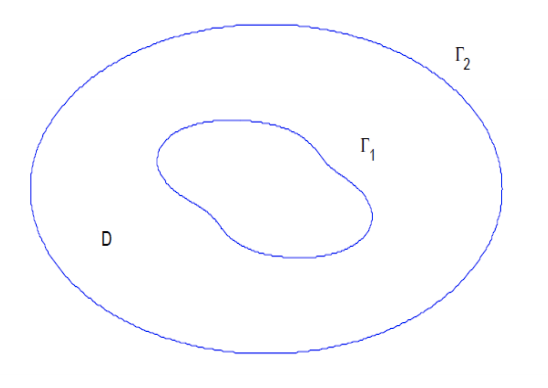
\includegraphics[width=0.55\textwidth]{resources/doubly-connected-region}
		\caption{}
		\label{fig:double-connected-region}
	\end{figure}

	Мішана задача Діріхле-Неймана для рівняння Лапласа полягає в знаходженні такої функції $u(x_1, x_2) \in C^{2}(D) \cup  C^{1}(\overline{D})$ що задовольняє

	\begin{enumerate}
		\item
		Рівняння Лапласа: 
		\begin{equation}
			\label{laplace-eq}
			\Delta{u} = 0 \quad \text{в} \quad D
		\end{equation}

		\item
		Граничні умови:
		\begin{equation}
			\label{dirichlet-condition}
			u = f_1, \quad (x_1, x_2) \in \Gamma_1,
		\end{equation}
	
		\begin{equation}
			\label{neumann-condition}
			\pdv{u}{v} = f_2, \quad (x_1, x_2) \in \Gamma_2,		
		\end{equation}

	\end{enumerate}
	де $v = v(x)$ - одиничний вектор зовнішньої нормалі, (\ref{dirichlet-condition}) є умовою Діріхле, а (\ref{neumann-condition}) є умовою Неймана.
	
\newcommand{\boundprob}{(\ref{laplace-eq}) -- (\ref{neumann-condition})} 
	
	
 \thispagestyle{empty}
 \section{Коректність задачі}
 ...
 
 %\subsection{Існування розв'язку}
 \subsection{Єдиність розв'язку задачі}
 \hspace{0.5cm}\theorem{green} Нехай $D$ - область з межею $\partial D \in C^1$ i $\overrightarrow{\nu} -$ одиничний вектор зовнішньої нормалі до межі $\partial D$. Тоді для $u \in C^1(\overline{D})$ і $v \in C^2(\overline{D})$ має місце перша формула Гріна
 $$
 \int_{D}(u \Delta v+grad u \cdot grad v) d x=\int_{\partial D} u \frac{\partial v}{\partial \nu} d s
 $$
 i для $u, v \in C^{2}(\overline{D})$ має місце друга формула Гріна
 $$
 \int_{D}(u \Delta v-v \Delta u) d x=\int_{\partial D}\left(u \frac{\partial v}{\partial \nu}-v \frac{\partial u}{\partial \nu}\right) d s
 $$
 
 \proof Посилання на Креса.
 
 
 \theorem{single-sol} Нехай $\Gamma_{1}, \Gamma_{2}$ -- гладкі границі, що належать класу $C^1$, обмежують двозв'язну (а може ні?) область $D$. Тоді задача \boundprob \space має на D (може замикання?) не більше одного розв'язку.
 
 \proof Від супротивного. Нехай $\exists u_1, u_2 \in C^{2}(\overline{D}): u_1 \neq u_2 $ -- два різні розв'язки задачі \boundprob. Запишемо цю задачу для функції $u^* = u_1 - u_2$:
 $$
 \Delta u^* = \Delta u_1 - \Delta u_2 = 0
 $$
 $$
 u^* = u_1 - u_2 = f_1 - f_1 = 0 \quad \text{на} \quad \Gamma_1
 $$
 $$
 \frac{\partial u^*}{\partial \nu}
 = \frac{\partial u_1}{\partial \nu} - \frac{\partial u_2}{\partial \nu}
 = f_2 - f_2 = 0 \quad \text{на} \quad \Gamma_2
 $$
 Застосуємо першу формулу Гріна з теореми \ref{green} при $u = v = u^*$:
 $$
 \int_{D}(\operatorname{grad} u^*)^2 dx
 = \int_{\partial D} u^* \frac{\partial u^*}{\partial \nu} dS
 - \int_{D} u^* \Delta u^* dx
 $$
 Тут $\partial D = \Gamma_1 \cup \Gamma_2$. Так як $\Delta u^* = 0 $ (чи ні?) на $D$, $u^*=0$ на $\Gamma_1$ і $\frac{\partial u^*}{\partial \nu} = 0$ на $\Gamma_2$, то отримуємо рівність
 $$
 \int_{D}(\operatorname{grad} u^*)^2 dx = 0,
 $$
 з якої випливає, що $\frac{\partial u^*}{\partial x_1} = 0$ і $\frac{\partial u^*}{\partial x_2} = 0$ на всій області $D$, тобто $u^* = \operatorname{const}$. Функція $u^*$ неперервна на $\overline{D}$ і $u^*=0$ на $\Gamma_1 \subset \overline{D}$, отже $u^*\equiv0 \Rightarrow u_1\equiv u_2$, що суперечить початковому припущенню. $\blacksquare$
 
 \thispagestyle{empty}
 \section{Зведення до інтегрального рівняння}
 
 \section{Коректність інтегрального рівняння}
 
 \section{Чисельне розв'язування}
 \subsection{Похибка}
 
 \section{Якийсь приклад}
 
	
 \end{document}
 
 